\chapter{Getting started}

\section{Introduction}

This chapter gives an overview of how \dfastmi can be used.
The program can run in two modes\footnote{\label{fn:backward1}The program still includes a third mode for backward compatibility, the so-called \emph{cli mode}, activated by means of \keyw{-{}-mode cli} on the command line.
This option is described in \Autoref{Chp:backward}.}:

\begin{enumerate}
\item \emph{batch mode}: in this mode the program runs the analysis without user interaction for a configuration file of which the name as command line argument,
\item \emph{gui mode}: in this mode the user specifies the configuration via a graphical user interface from which the analysis can either be started directly or the configuration can be saved for batch mode execution at a later time.
\end{enumerate}

The program runs by default in the gui mode; other run modes can be selected via the command line argument.

\begin{tabular}{l|l|p{8cm}}
short & long & description \\ \hline
\keyw{-h} & \keyw{-{}-help} & show help text and exit \\
 & \keyw{-{}-rivers} & name of river configuration file (default: \keyw{Dutch\_rivers.ini}) \\
 & \keyw{-{}-language} & language selection: \keyw{NL} or \keyw{UK} (default: \keyw{UK}) \\
 & \keyw{-{}-mode} & run mode \keyw{batch}, \keyw{cli}\footref{fn:backward1} or \keyw{gui} (default: \keyw{gui} \\
 & \keyw{-{}-config} & name of analysis configuration file \\
\end{tabular}

By default the program runs for the Dutch Rhine and Meuse river branches, but a different river configuration can be provided by means of the \keyw{-{}-rivers} command line switch; this option is supported by all run modes.
For details on the format of the river configuration file, see the appropriate section in the appendix.
The language setting influences all texts displayed by the program as well as the texts written to the report file as well as the names of the various output files.
The following list indicates the English and Dutch names:

\begin{itemize}
\item Text file with summary report of the analysis \\
English: \keyw{report.txt} \\
Dutch: \keyw{verslag.run}
\item UGRID netCDF file containing variables for average yearly change, maximum change, and minimum change (when the analysis runs using \dflowfm input) \\
English: \keyw{dfastmi\_results.nc} \\
Dutch: \keyw{dfastmi\_resultaten.nc}
\end{itemize}

The following sections describe the different execution modes.

\section{Running in batch mode}

The batch mode runs an analysis using \dflowfm results without user interaction, old WAQUA files are no longer supported.
The program should be started with the run mode set to \keyw{batch} and a configuration file specified on the command line as follows

\begin{Verbatim}
> dfastmi --mode batch --config myfile.cfg
\end{Verbatim}

You may choose to run the program in either Dutch \keyw{-{}-language NL} or English \keyw{-{}-language UK}; the latter is the default.
Please note that the language does not only affect the text in the report, but also the names of the output files as indicated in the opening section of this chapter.
The content of the configuration file is described in \Autoref{app:config}; it can be generated using either a text editor or \dfastmi running in gui mode.

\section{Running in gui mode}

This is the default mode for the program, so no command line argument needed.
The gui works only with the newer \dflowfm result files.
As with the other run modes, you may choose to run the program in either Dutch \keyw{-{}-language NL} or English \keyw{-{}-language UK}; the latter is the default.
Please note that the language does not only affect the text in the report, but also the names of the output files as indicated in the opening section of this chapter.
Furthermore, you may specify a configuration file to load upon start.
For example

\begin{Verbatim}
> dfastmi --language NL --config myfile.cfg
\end{Verbatim}

runs the program in Dutch and loads the myfile.cfg configuration file into the graphical user interface.

\begin{figure}
\center
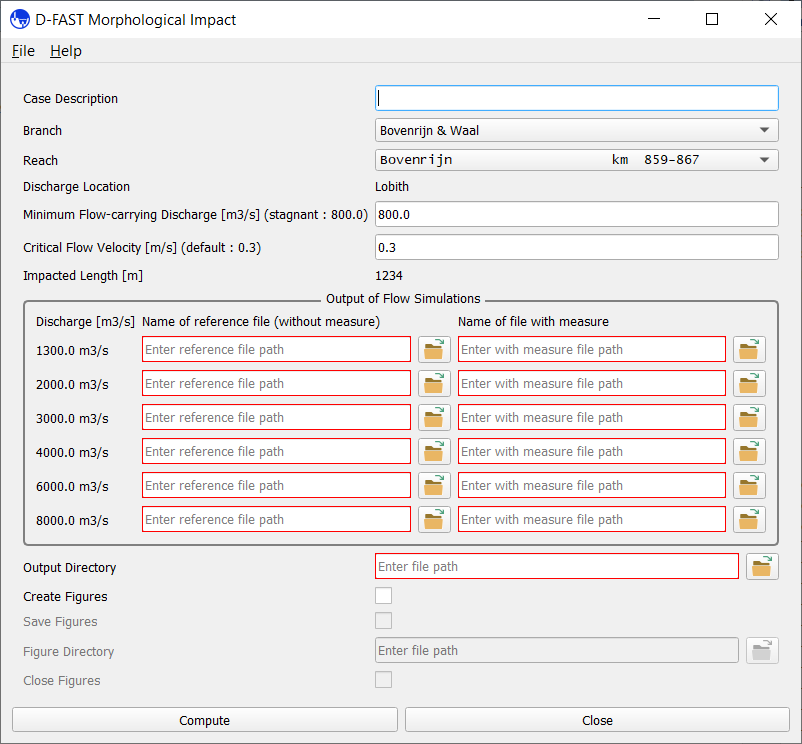
\includegraphics[width=12cm]{figures/main_dialog.png}
\caption{Example of the main dialog}
\end{figure}

The following text describes the functionality of the graphical user interface from top to bottom.
The \keyw{File} menu provides access to options to load a configuration file and to save the current selection in the gui to a configuration file.
The \keyw{Help} menu provides access to about boxes for \dfastmi itself and for the PyQt5 graphical framework.

As a user, you start specifying the branch and reach of the study.
Changing this selection will affect all fields below overwriting any previously entered values.
You have to specify the minimum flow-carrying discharge of the measure.
Together with the branch and reach selection, this determines the distance over which the river branch may be affected during the first year.
This length \unitbrackets{m} is indicated, and dynamically updated with each change you make.

Subsequently, you are presented with a list of flow conditions for which you need to provide data files representing the reference situation and the situation with the measure implemented.
The names of the files need to be specified in the edit fields below.

The last input item for the analysis is the critical flow velocity \unitbrackets{m/s} for sediment transport.
Finally, we find at the bottom of the dialog some options for the output of the \dfastmi run, and a button to run the analysis in the folder from which the program was started, and a button to end the program.

\section{Running from Python source code}
It's recommended to run \dfastmi as binary, but you may also run it directly from the Python source code.
The source code can be downloaded from \url{https://github.com/Deltares/D-FAST_Morphological_Impact}; please check which source code version you need.
A Python Poetry\footnote{\url{https://python-poetry.org/}} environment has been configured to relatively easily install all libraries necessary for running the tool.
Follow the steps in the online Developer user starter guide to set up the run environment using \keyw{poetry install}.
In that case the program can be started from the command prompt as

\begin{Verbatim}
poetry run python -m dfastmi ...options...
\end{Verbatim}

or from within a running Python environment as

\begin{Verbatim}
import dfastmi.cmd
dfastmi.cmd.run()
\end{Verbatim}

where optionally the \command{language} (default \command{UK}), \command{runmode} (default \command{GUI}), \command{configfile} (default \command{dfastmi.cfg}) and \command{rivers\_file} (default \command{Dutch\_rivers.ini}) can be specified as arguments.